\documentclass{article}[18pt]
\ProvidesPackage{format}
%Page setup
\usepackage[utf8]{inputenc}
\usepackage[margin=0.7in]{geometry}
\usepackage{parselines} 
\usepackage[english]{babel}
\usepackage{fancyhdr}
\usepackage{titlesec}
\hyphenpenalty=10000

\pagestyle{fancy}
\fancyhf{}
\rhead{Sam Robbins}
\rfoot{Page \thepage}

%Characters
\usepackage{amsmath}
\usepackage{amssymb}
\usepackage{gensymb}
\newcommand{\R}{\mathbb{R}}

%Diagrams
\usepackage{pgfplots}
\usepackage{graphicx}
\usepackage{tabularx}
\usepackage{relsize}
\pgfplotsset{width=10cm,compat=1.9}
\usepackage{float}

%Length Setting
\titlespacing\section{0pt}{14pt plus 4pt minus 2pt}{0pt plus 2pt minus 2pt}
\newlength\tindent
\setlength{\tindent}{\parindent}
\setlength{\parindent}{0pt}
\renewcommand{\indent}{\hspace*{\tindent}}

%Programming Font
\usepackage{courier}
\usepackage{listings}
\usepackage{pxfonts}

%Lists
\usepackage{enumerate}
\usepackage{enumitem}

% Networks Macro
\usepackage{tikz}


% Commands for files converted using pandoc
\providecommand{\tightlist}{%
	\setlength{\itemsep}{0pt}\setlength{\parskip}{0pt}}
\usepackage{hyperref}

% Get nice commands for floor and ceil
\usepackage{mathtools}
\DeclarePairedDelimiter{\ceil}{\lceil}{\rceil}
\DeclarePairedDelimiter{\floor}{\lfloor}{\rfloor}

% Allow itemize to go up to 20 levels deep (just change the number if you need more you madman)
\usepackage{enumitem}
\setlistdepth{20}
\renewlist{itemize}{itemize}{20}

% initially, use dots for all levels
\setlist[itemize]{label=$\cdot$}

% customize the first 3 levels
\setlist[itemize,1]{label=\textbullet}
\setlist[itemize,2]{label=--}
\setlist[itemize,3]{label=*}

% Definition and Important Stuff
% Important stuff
\usepackage[framemethod=TikZ]{mdframed}

\newcounter{theo}[section]\setcounter{theo}{0}
\renewcommand{\thetheo}{\arabic{section}.\arabic{theo}}
\newenvironment{important}[1][]{%
	\refstepcounter{theo}%
	\ifstrempty{#1}%
	{\mdfsetup{%
			frametitle={%
				\tikz[baseline=(current bounding box.east),outer sep=0pt]
				\node[anchor=east,rectangle,fill=red!50]
				{\strut Important};}}
	}%
	{\mdfsetup{%
			frametitle={%
				\tikz[baseline=(current bounding box.east),outer sep=0pt]
				\node[anchor=east,rectangle,fill=red!50]
				{\strut Important:~#1};}}%
	}%
	\mdfsetup{innertopmargin=10pt,linecolor=red!50,%
		linewidth=2pt,topline=true,%
		frametitleaboveskip=\dimexpr-\ht\strutbox\relax
	}
	\begin{mdframed}[]\relax%
		\centering
		}{\end{mdframed}}



\newcounter{lem}[section]\setcounter{lem}{0}
\renewcommand{\thelem}{\arabic{section}.\arabic{lem}}
\newenvironment{defin}[1][]{%
	\refstepcounter{lem}%
	\ifstrempty{#1}%
	{\mdfsetup{%
			frametitle={%
				\tikz[baseline=(current bounding box.east),outer sep=0pt]
				\node[anchor=east,rectangle,fill=blue!20]
				{\strut Definition};}}
	}%
	{\mdfsetup{%
			frametitle={%
				\tikz[baseline=(current bounding box.east),outer sep=0pt]
				\node[anchor=east,rectangle,fill=blue!20]
				{\strut Definition:~#1};}}%
	}%
	\mdfsetup{innertopmargin=10pt,linecolor=blue!20,%
		linewidth=2pt,topline=true,%
		frametitleaboveskip=\dimexpr-\ht\strutbox\relax
	}
	\begin{mdframed}[]\relax%
		\centering
		}{\end{mdframed}}
\lhead{MCS - Logic and Discrete Structures}


\begin{document}
\begin{center}
\underline{\huge Sets}
\end{center}

\section{Some notation}
\begin{itemize}
	\item We write $x\in X$ to denote that x is an element or member of the set X, or that X contains x, with $x\notin X$ denoting that x is not an element of X
	\item We can describe a set by listing it's elements
	\begin{itemize}
		\item the set of pairs of prime numbers less than 6 is $\{\{2,3\}\{2,5\},\{3,5\}\}$
	\end{itemize}
	\item It is always possible if a set is finite
	\item However if a set is infinite, then it is not possible, unless we cheat by adding dots
	\item We often describe a set by it's defining property, e.g.:
	\begin{itemize}
		\item The set of natural numbers $\mathbb{N}=\{x: x \ \textrm{x is a natural number\} = \{0,1,2,...\}}$
		\item The set of integers $\mathbb{Z}=\{ x : x \in N \text { or } x = - y \text { for } y \in \mathbf { N } \} = \{ 0,1 , - 1,2 , - 2 , \ldots \}$
		\item The set of rational numbers $\mathbb{Q}=\{ x : x = y / z \text { for } y , z \in \mathbf { Z } \text { with } z \neq 0 \}$
		\item The set of real numbers $\mathbb{R}=\{ x : x \text { is a real number } \}$
	\end{itemize}
	\item We regard 0 as a natural number
\end{itemize}
\section{Cardinality}
\begin{itemize}
	\item If there are exactly n distinct elements in the set S, where $n\in \mathbf{ N }$ then S is finite and has size or cardinality n and we write $|S|=n$
	\begin{itemize}
		\item As we remarked earlier, if S is not finite then it is infinite
	\end{itemize}
	\item Of course, the empty set $\varnothing$ has size 0
	\item We can also define the size of an infinite set
	\item One might be tempted to think that all infinite sets have the same size, however there are different sizes of infinity
\end{itemize}
\section{Set Equality}
\begin{itemize}
	\item Two sets X and Y are equal when we write $X=Y$ iff they contain exactly the same elements
	\item Equivalently X and Y are equal iff:
	\begin{itemize}
		\item for every object x, $x\in X$ implies that $x\in Y$
		\item for every object x $x\in Y$ implies that $x\in X$
		\item For example:
		\begin{itemize}
			\item $\{1,2,3,4,5\}={3,2,4,5,1}$
		\end{itemize}
	\end{itemize}
	\item \textbf{Singleton Set} - A set containing exactly one element
	\item Note that strictly speaking $\{1,3,3,5\}$ is not a set but a multiset, but we regard it as a description of the set $\{1,3,5\}$
	\item Recall also that our sets are objects and so we can have sets containing sets as elements, indeed, we can have sets containing sets as elements, e.g.
	\begin{itemize}
		\item $\{\varnothing\}\neq \varnothing$
		\item $\{\{\varnothing\}\}\neq \{\varnothing\}$ 
	\end{itemize}
\end{itemize}
\section{Venn Diagrams}
\begin{itemize}
	\item Sometimes it is useful to have a pictoral representation of a set or sets
	\item Any venn diagram is contained within (usually) a rectangle, depicting the set of all objects
	\item Sets are represented by circles and elements by points or items
\end{itemize}
\begin{center}
	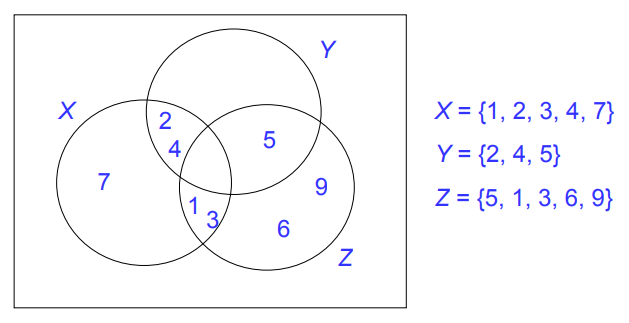
\includegraphics[scale=0.7]{venn}
\end{center}
\section{Subsets}
\begin{itemize}
	\item A set X is a subset of set Y when we write $X\subseteq Y$ iff every element that is in X is also in Y
	\item So, X is not a subset of Y, when we write $X\subsetneq Y$ iff there is some element that is in X that is not in Y
	\item A subset X of Y is a proper subset when we write $X\subset Y$, if $X\subseteq Y$ and there may be at least one element of Y that is not in X
\end{itemize}
\begin{center}
	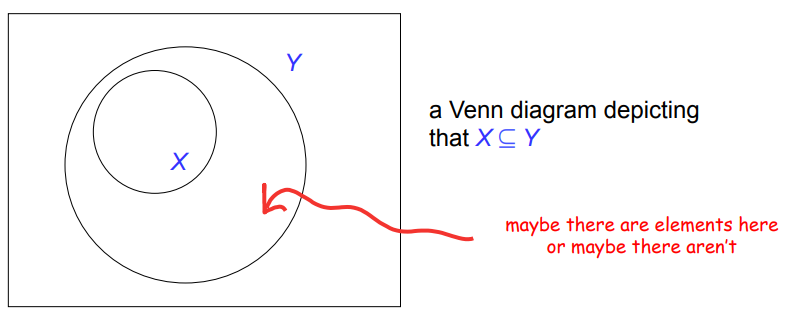
\includegraphics[scale=0.7]{venn1}
\end{center}
\section{Some facts about subsets}
\begin{itemize}
	\item $\mathbb{N}\subset \mathbb{Z}\subset \mathbb{Q}\subset \mathbb{R}$
	\item For any set S $S\subseteq S$
	\item For any set S $\varnothing\subseteq S$
	\item For any sets A and B
	\begin{itemize}
		\item $A=B$ iff $A\subseteq B$ and $B\subseteq A$
		\begin{itemize}
			\item Trivially if $A=B$ then $A\subseteq B$ and $B\subseteq A$
			\item Conversely suppose that $A\subseteq B$ and $B\subseteq A$
			\begin{itemize}
				\item If $x\in A$ then $x\in B$
				\item If $x\notin A$ then $x\notin B$
			\end{itemize}
			\item So A=B
		\end{itemize}
	\end{itemize}
	\item For every set A if $A\subseteq \varnothing$ then $A=\varnothing$
	\begin{itemize}
		\item Suppose that $A\subseteq \varnothing$ and let $x\in A$, so $x\in \varnothing$, a contradiction
	\end{itemize}
\end{itemize}
\section{The Power Set}
\begin{itemize}
	\item There are a number of common operations upon sets which enable us to create new sets out of old ones
	\item Let S be a set. The \textbf{power set} P(S) (or P(S) or $2^s$) is the set of all subsets of S
	\item We already have seen that every non empty set S has at least 2 subsets, $\varnothing$ and S
	\item However, in general, there are many more subsets, e.g:
	\begin{itemize}
		\item If $S=\{0,1,2,3\}$ then P(S) is all combinations of 0,1,2,3 and the empty set
		\item If $S=\mathbb{N}$ then P(S) is any set of natural numbers
		\item If $S=\varnothing$ then:
		\begin{itemize}
			\item $P(S)=\{\varnothing\}$
			\item $P(P(S))=\{\varnothing,\{\varnothing\}\}$
			\item $P(P(P(S)))=\{ \varnothing , \{ \varnothing \} , \{ \{ \varnothing \} \} , \{ \varnothing , \{ \varnothing \} \} \}$
		\end{itemize}
	\end{itemize}
	\item In general, if S is finite of size n, then $P(S)$ is finite of size $2^n$
\end{itemize}
\section{The Cartesian Product}
\begin{itemize}
	\item Often, the order of a collection of elements matters, though the order of the elements in a set is of no importance
	\item An ordered n-touple $(a_1,a_2,...,a_n)$ is an ordered collection of elements
	\item If $n=2(resp. n=3)$ then we call the touple an ordered pair (resp touple)
	\item Two ordered n touples are equal iff $a_i=b_i$ for all $i=1,2,...,n$
	\item Cartesian products allow us to talk about "order"
	\item For any two sets X and Y, the cartesian product $X\times Y$ is the set
	$$\{ ( x , y ) : x \in X \text { and } y \in Y \}$$
	\item For example:
	\begin{itemize}
		\item The Cartesian product of $\{0,1,2\}$ and $\{a,b\}$ is
		$$\{ ( 0 , a ) , ( 1 , a ) , ( 2 , a ) , ( 0 , b ) , ( 1 , b ) , ( 2 , b ) \}$$
		\item The Cartesian product of $\{a,b\}$ and $\{0,1,2\}$ is:
		$$\{ ( a , 0 ) , ( a , 1 ) , ( a , 2 ) , ( b , 0 ) , ( b , 1 ) , ( b , 2 ) \}$$
	\end{itemize}
	\item We can also define the Cartesian product of more than two sets
	\item Let $A_1,A_2,...,A_n$ be sets. The Cartesian product $A_1\times A_2 \times ...\times A_n$ is the set:
	$$\left\{ \left( a _ { 1 } , a _ { 2 } , \dots , a _ { n } \right) : a _ { i } \in A _ { i } , \text { for all } i = 1,2 , \ldots , n \right\}$$
	\item If $A_1,A_2,...,A_n$ are all finite sets with $|A_i|=m_i$ for $i=1,2,...,n$ then:
	$$\left| A _ { 1 } \times A _ { 2 } \times \ldots \times A _ { n } \right| = m _ { 1 } \times m _ { 2 } \times \ldots \times m _ { n }$$
\end{itemize}
\section{Union and Intersection}
\begin{itemize}
	\item Let A and B be sets, the union of A and B, written as $A\cup B$ is the set that contains all elements that are in A, in B or both
	\begin{itemize}
		\item That is $A \cup B = \{ x : x \in A \vee x \in B \}$
	\end{itemize}
	\item Let A and B be sets. The intersection of A and B, written $A \cap B$ is the set of elements that are in A and B
	\begin{itemize}
		\item That is, $A \cap B = \{ x : x \in A \wedge x \in B \}$
	\end{itemize}
	\item Two sets are called disjoint if their intersection is the empty set
		\item Principle of inclusion-exclusion: if A and B are finite sets then:
		$$| A \cup B | = | A | + | B | - | A \cap B |$$
\end{itemize}
\subsection{Union and Intersection Venn Diagrams}
\begin{center}
	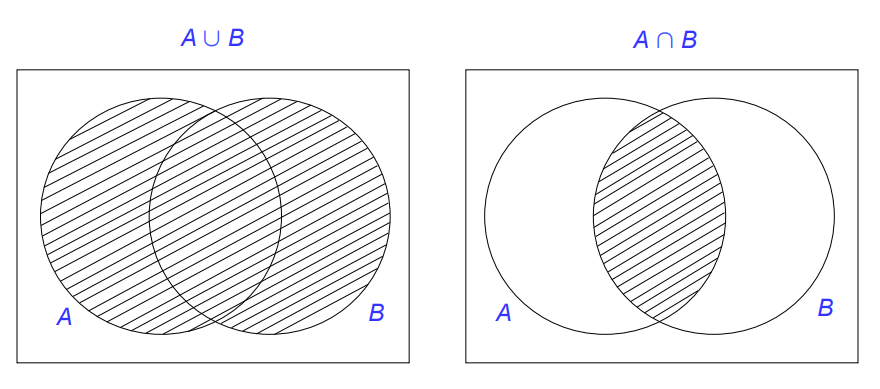
\includegraphics[scale=0.7]{venn2}
\end{center}
\section{Difference and Compliment}
\begin{itemize}
	\item Let A and B be sets. The difference of A and B, written $A-B (or  \ A\backslash B)$ is the set that contains all elements that are in A but not in B
	\begin{itemize}
		\item That is, $A - B = \{ x : x \in A \wedge x \notin B \}$
	\end{itemize}
	\item Let A be a set. The compliment of A, written $\overline{A}$ is the set that contains all elements that are not in A
	\begin{itemize}
		\item That is, $A = \{ x : x \notin A \}$
	\end{itemize}
	\item The difference A-B is sometimes called the \textbf{complement of B with respect to A}
\end{itemize}
\subsection{Venn Diagram of Difference and Complement}
\begin{center}
	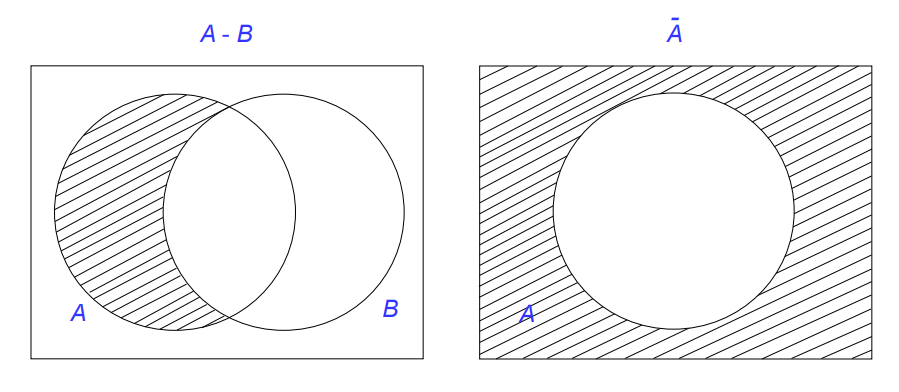
\includegraphics[scale=0.7]{venn3}
\end{center}
\section{A Different Semantics}
\begin{itemize}
	\item Note that we can define different semantics for propositional logic
	\item Consider some formula $\phi$ of propositional logic such as:
	$$( X \wedge ( Y \wedge Z ) ) \vee \neg ( \neg X \vee ( Y \wedge Z ) )$$
	\item Previously we interpreted $\phi$ using truth assignments, with a truth assignment making $\phi$ either true or false
	\item We can interpret $\phi$ by assigning sets to each of the propositional variables:
	\begin{itemize}
		\item We get that $\phi$ denotes a set of elements via:
		\begin{itemize}
			\item Interpret $\land$ as intersection
			\item Interpret $\lor$ as union
			\item Interpret $\lnot$ as complement
		\end{itemize}
	\end{itemize}
	\item Write $\phi\equiv_s\psi$  iff $\phi$ and $\psi$ always denote the same set of elements
	\item We get the identities from propositional logic
	$$\phi \equiv _ { S } \psi \text { if, and only if, } \phi \equiv \psi$$
	\item So $( X \wedge ( Y \wedge Z ) ) \vee \neg ( \neg X \vee ( Y \wedge Z ) )$ denotes the set of elements shown, i.e. X
\end{itemize}
\begin{center}
	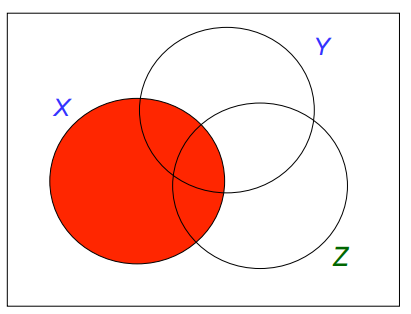
\includegraphics[scale=0.7]{venn4}
\end{center}

\end{document}